\documentclass{article}
\usepackage[utf8]{inputenc}
\usepackage[dutch]{varioref}
\usepackage[autostyle]{csquotes} 
\usepackage[dutch]{babel}
\usepackage{listings}
\usepackage{pdfpages}
\usepackage{url}
\usepackage{natbib}
\usepackage{graphicx}

\title{Stageverslag}
\author{\mbox{Pieter-Jan} Robrecht}
\date{Maart 2016}

\begin{document}

%\maketitle
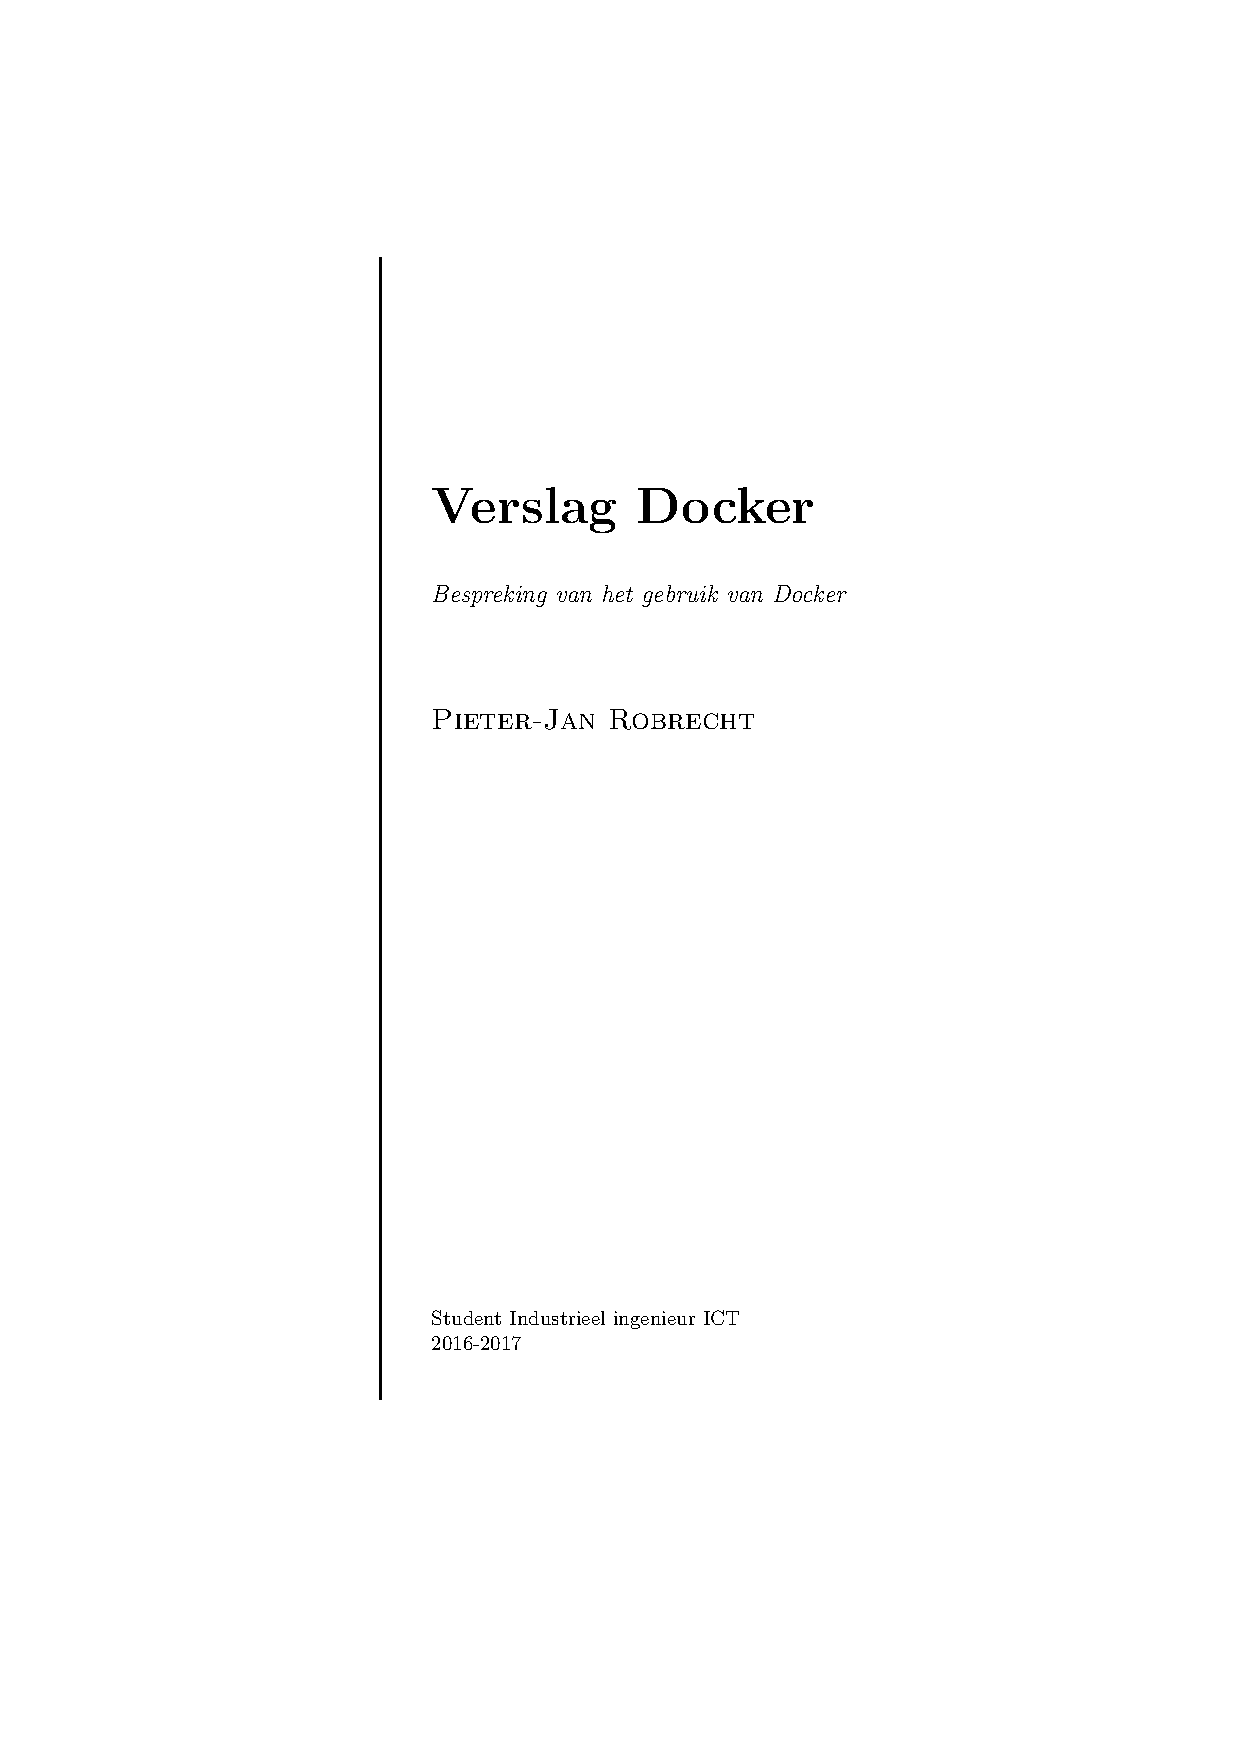
\includepdf{titel/titeldocker.pdf}

%Volgende lijn is om de titelpagina geen paginanummer te geven
\clearpage
\setcounter{page}{1}

\tableofcontents
\lstlistoflistings
\clearpage

\section{Inleiding}
Het doel van dit verslag is het bespreken van Docker als mogelijke oplossing voor het Python Framework Installer probleem.
Voor het bespreken van Docker ging ik op een gelijkaardige manier te werk als tijdens mijn stage.
Ik heb de tool uitgeprobeerd en ik wou een installer maken die het volgende moest kunnen:
\begin{itemize}
\item het uitvoeren van een executable
\item het uitpakken van een zip bestand
\item het uitvoeren van de setup.py horende bij het zip bestand
\end{itemize}
Verder heb ik ook gekeken wat de mogelijkheden zijn voor het uitvoeren van een update.
Docker maakt gebruik van images (read-only templates met instructies) voor het opzetten van verschillende containers.
Deze containers zijn dan uitvoerbare instanties van de image \citep{docker}.

\section{Bespreking}
Al snel blijkt dat Docker verschillende plus- maar ook minpunten heeft.
Zo is het bijvoorbeeld enkel mogelijk om Docker te installeren op een computer met Windows 10 Professional, Enterprise (Anniversary Edition) of Windows server 2016 \citep{microsoft}.
Docker heeft Hyper-V nodig om te kunnen werken op Windows \citep{dockerNodig}.
Gelukkig kon ik wel gebruik maken van de Docker toolbox waarmee ik dan aan de slag kon.
Jammer genoeg kon ik met de toolbox versie van Docker geen Windows containers maken, enkel Linux containers.
In listing~\vref{list:dockerfile} kan u zien dat ik als base image Ubuntu heb gekozen.
Aangezien de base image Ubuntu is, is het niet mogelijk om Windows executables uit te voeren.
Hiernaast was het ook niet mogelijk om de setup.py uit te voeren aangezien deze geschreven is voor Windows systemen.
Het installeren en opzetten van de omgeving ging wel vlot en verliep verder zonder problemen.

Een voordeel van Docker is de mogelijk tot het gebruiken van repositories.
Hierdoor wordt het mogelijk om een systeem gelijkaardig aan GIT op te bouwen.
Een image kan worden aangepast en worden opgeslagen onder een specifieke tag, gebruikers kunnen vervolgens kiezen welke versie van de image ze downloaden en uitvoeren in een container.
Er kan ook zeer eenvoudig gewisseld worden tussen verschillende versies.

\section{Besluit}
We kunnen dus besluiten dat Docker verschillende voordelen heeft die aantrekkelijk zijn.
De repositories, het direct kunnen deployen van een omgeving, ... zijn allemaal zeer sterke pluspunten van Docker.
Het grootste nadeel, momenteel, is dat Docker Hyper-V nodig heeft om te kunnen draaien op Windows computers.
Docker zou kunnen draaien op Windows 10 Professional, Enterprise (Anniversary Edition) of Windows server 2016.
Aangezien ik niet over deze versies van Windows 10 beschikte en dat de laatste nog niet beschikbaar is, was het niet mogelijk om de Windows containers van Docker uit te testen.
Het is dus niet geweten in hoeverre Docker een oplossing zou kunnen bieden voor het probleem.

Aan de andere kant zouden de Linux containers wel een degelijke oplossing kunnen bieden voor het probleem.
Ze geven een robuuste indruk en door het repository systeem zou er snel en eenvoudig gewisseld kunnen worden tussen verschillende versies.
De huidige installatiemethode zou dan wel moeten aangepast worden aangezien Linux niet overweg kan met de verschillende executables.

\section{Code}
\lstinputlisting[caption={Docker Dockerfile}, label={list:dockerfile}]{../code/docker/test/dockerfile.txt}

%Alfabetische volgorde
%\bibliographystyle{plain}
%Orde van bib file
\bibliographystyle{unsrt}
\bibliography{bib/dockerbib}

\end{document}